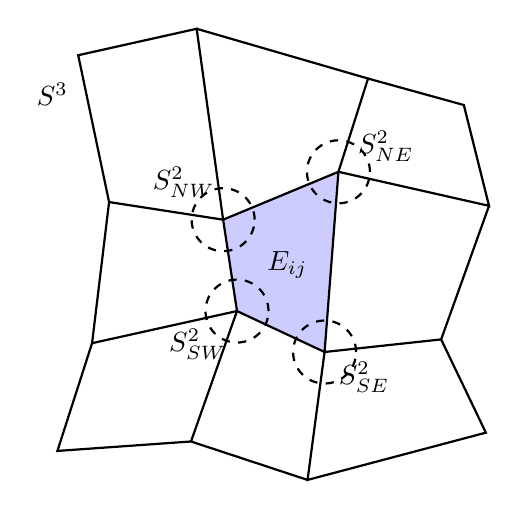
\begin{tikzpicture}[xscale=1.6, yscale = 1.6]
    \coordinate(P0) at (-0.225,0.025);
    \coordinate(P1) at (0.835,0.1);
    \coordinate(P2) at (1.76,-0.205);
    \coordinate(P3) at (3.175,0.17);
    \coordinate(P4) at (0.05,0.88);
    \coordinate(P5) at (1.2,1.135);
    \coordinate(P6) at (1.895,0.81);
    \coordinate(P7) at (2.82,0.91);
    \coordinate(P8) at (0.185,2);
    \coordinate(P9) at (1.09,1.86);
    \coordinate(P10) at (2.005,2.24);
    \coordinate(P11) at (3.2,1.97);
    \coordinate(P12) at (-0.06,3.165);
    \coordinate(P13) at (0.88,3.375);
    \coordinate(P14) at (2.24,2.98);
    \coordinate(P15) at (3,2.77);
    
    \draw [thick,-,fill=blue, fill opacity=0.2] (P5) -- (P6) -- (P10) -- (P9) -- cycle;
    \draw [thick,-] (P5) -- (P4) -- (P8) -- (P9);
    \draw [thick,-] (P9) -- (P13)-- (P12) -- (P8);
    \draw [thick,-] (P13)-- (P14)-- (P10);
    \draw [thick,-] (P14)-- (P15)-- (P11) -- (P10);
    \draw [thick,-] (P11)-- (P7)-- (P6);
    \draw [thick,-] (P6)-- (P2)-- (P3) -- (P7);
    \draw [thick,-] (P2)-- (P1) -- (P5);
    \draw [thick,-] (P1)-- (P0)-- (P4);
    
    \draw [thick, dashed] (P6) circle (.25cm);
    \draw [thick, dashed] (P5) circle (.25cm);
    \draw [thick, dashed] (P10) circle (.25cm);
    \draw [thick, dashed] (P9) circle (.25cm);
    
    \draw [thick] (1.6, 1.5) node[]{$E_{ij}$};
    
    \draw [thick] (P6) node[below, xshift = .5cm, yshift = -.0cm]{$S^2_\text{SE}$};
    \draw [thick] (P5) node[below, xshift = -.5cm, yshift = -.1cm]{$S^2_\text{SW}$};
    \draw [thick] (P9) node[above, xshift = -.5cm, yshift = .15cm]{$S^2_\text{NW}$};
    \draw [thick] (P10) node[above, xshift = .6cm, yshift = .0cm]{$S^2_\text{NE}$};
    
    \draw [thick] (P12) node[left, yshift = -.5cm]{$S^3$};
  
\end{tikzpicture}
